\documentclass[11pt,letterpaper]{article}
\usepackage[lmargin=1in,rmargin=1in,tmargin=1in,bmargin=1in]{geometry}
\usepackage{../style/homework}
\usepackage{../style/commands}
\setbool{quotetype}{true} % True: Side; False: Under
\setbool{hideans}{true} % Student: True; Instructor: False

% -------------------
% Content
% -------------------
\begin{document}

\homework{9: Due 10/24}{You're a good boy, Jeff.}{Catherie Dahmer, \par Dahmer - Monster: \par The Jeffrey Dahmer Story}

% Problem 1
\problem{10} Let $f(x)$ be a function such that $f^{-1}(x)$ exists. A partial table of values for $f(x)$ is given below: \par
	\begin{table}[!ht]
	\centering
	\begin{tabular}{|r||c|c|c|c|c|} \hline 
	$x$ & $1$ & $2$ & $3$ & $4$ & $5$ \\ \hline
	$f(x)$ & $5$ & $7$ & $0$ & $9$ & $3$ \\ \hline
	\end{tabular}
	\end{table}
Based on the table above (or your knowledge of functions and inverses), find the following:
	\begin{enumerate}[(a)]
	\item $f(3)$
	\item $f^{-1}(3)$
	\item $f(4)$
	\item $f^{-1}(9)$
	\item $f(f^{-1}(5))$
	\item $f^{-1} \big( f(9) \big)$
	\item $f^{-1} \big( f(-8) \big)$
	\item $f \big( f^{-1}(10) \big)$
	\end{enumerate}



\newpage



% Problem 2
\problem{10} Let $f(x)= \frac{1}{4} (x - 3)$. Assume that $f^{-1}(x)$ exists. 
	\begin{enumerate}[(a)]
	\item Find $f(15)$. 
	\item Use (a) to explain why $f^{-1}(3)= 15$. 
	\item Solve the equation given by $f(x)= 11$.
	\item Use (c) to explain why $f^{-1}(11)= 2$. 
	\end{enumerate}



\newpage



% Problem 3
\problem{10} A graph of a relation $f(x)$ is shown below:
	\[
	\fbox{
	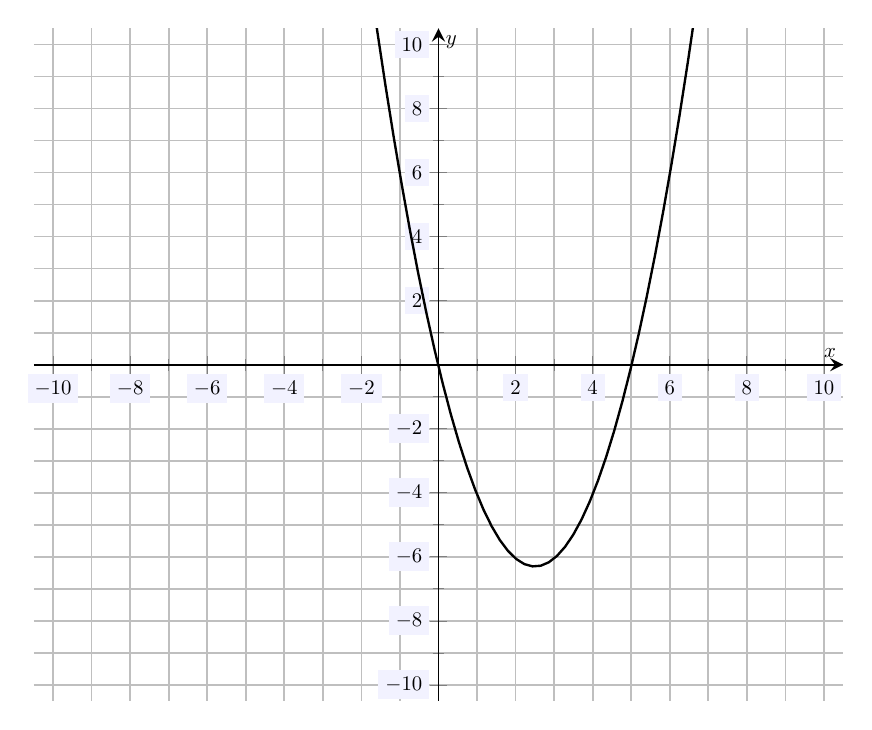
\begin{tikzpicture}[scale=1.5,every node/.style={scale=0.5}]
	\begin{axis}[
	grid=both,
	axis lines=middle,
	ticklabel style={fill=blue!5!white},
	xmin= -10.5, xmax=10.5,
	ymin= -10.5, ymax=10.5,
	xtick={-10,-8,-6,-4,-2,0,2,4,6,8,10},
	ytick={-10,-8,-6,-4,-2,0,2,4,6,8,10},
	minor tick = {-10,-9,...,10},
	xlabel=\(x\),ylabel=\(y\),
	]
	\addplot[line width= 0.02cm,samples=100,domain= -10.5:10.5] ({x},{(x - 2.5)^2 - 6.3}); 
	\end{axis}
	\end{tikzpicture}
	}
	\] 
Using the graph above, answer the following:
	\begin{enumerate}[(a)]
	\item Is the relation $f(x)$ a function? Explain.
	\item Does the relation $f(x)$ have an inverse function? Explain. 
	\end{enumerate}


\end{document}